\documentclass{beamer}

\usepackage{amsmath}
\usepackage{mathtools}
\usepackage{amsfonts}
\usepackage{amssymb}
\usepackage{url}
\usepackage{caption}
\usepackage{subcaption}
\usepackage{matlab-prettifier}

\renewcommand{\vec}[1]{\boldsymbol{\mathbf{#1}}} %vector, je potreba do budoucna nahradit za textbf
\newcommand{\mat}[1]{\mathbf{#1}} %matrix
\newcommand{\inner}[2]{\left \langle #1, #2 \right \rangle} %inner product 
\newcommand{\norm}[1]{\Vert #1 \Vert} %norm

\usetheme{Copenhagen}

\title{Modul pro sběr dat ze senzorů s rozhraním LoRa}
\author{Jiří Maňák}
\institute[]{vedoucí: prof. Ing. Radislav Šmíd, Ph. D.}
\date{\today}

\begin{document}


\begin{frame}
\titlepage
\end{frame}


\begin{frame}{Cíle semestrálního projektu}
\begin{itemize}
    \item Navrhnout a realizovat modul pro sběr dat ze senzorů fyzikálních veličin s rozhraním LoRa a mikrokontrolerem STM32
    \item Implementovat možnost OTA aktualizace firmware
    \item Prozkoumat možnosti napájení pro dlouhodobé venkovní použití
\end{itemize}
\end{frame}


\begin{frame}{Výsledky: hardware modulu}
\begin{columns}[T]
\begin{column}{.45\textwidth}
    \begin{itemize}
        \item Specifikace
        \item Výběr komponent
        \item Schema
        \item Návrh PCB
        \item Výroba
        \item Oživení
        \item Ověření funkčnosti
    \end{itemize}
    Zbývá
    \begin{itemize}
        \item Validace parametrů RF
        \item Charakterizace spotřeby
    \end{itemize}
\end{column}%
\hfill%
\begin{column}{.55\textwidth}
    \begin{figure}[h]
        \centering
        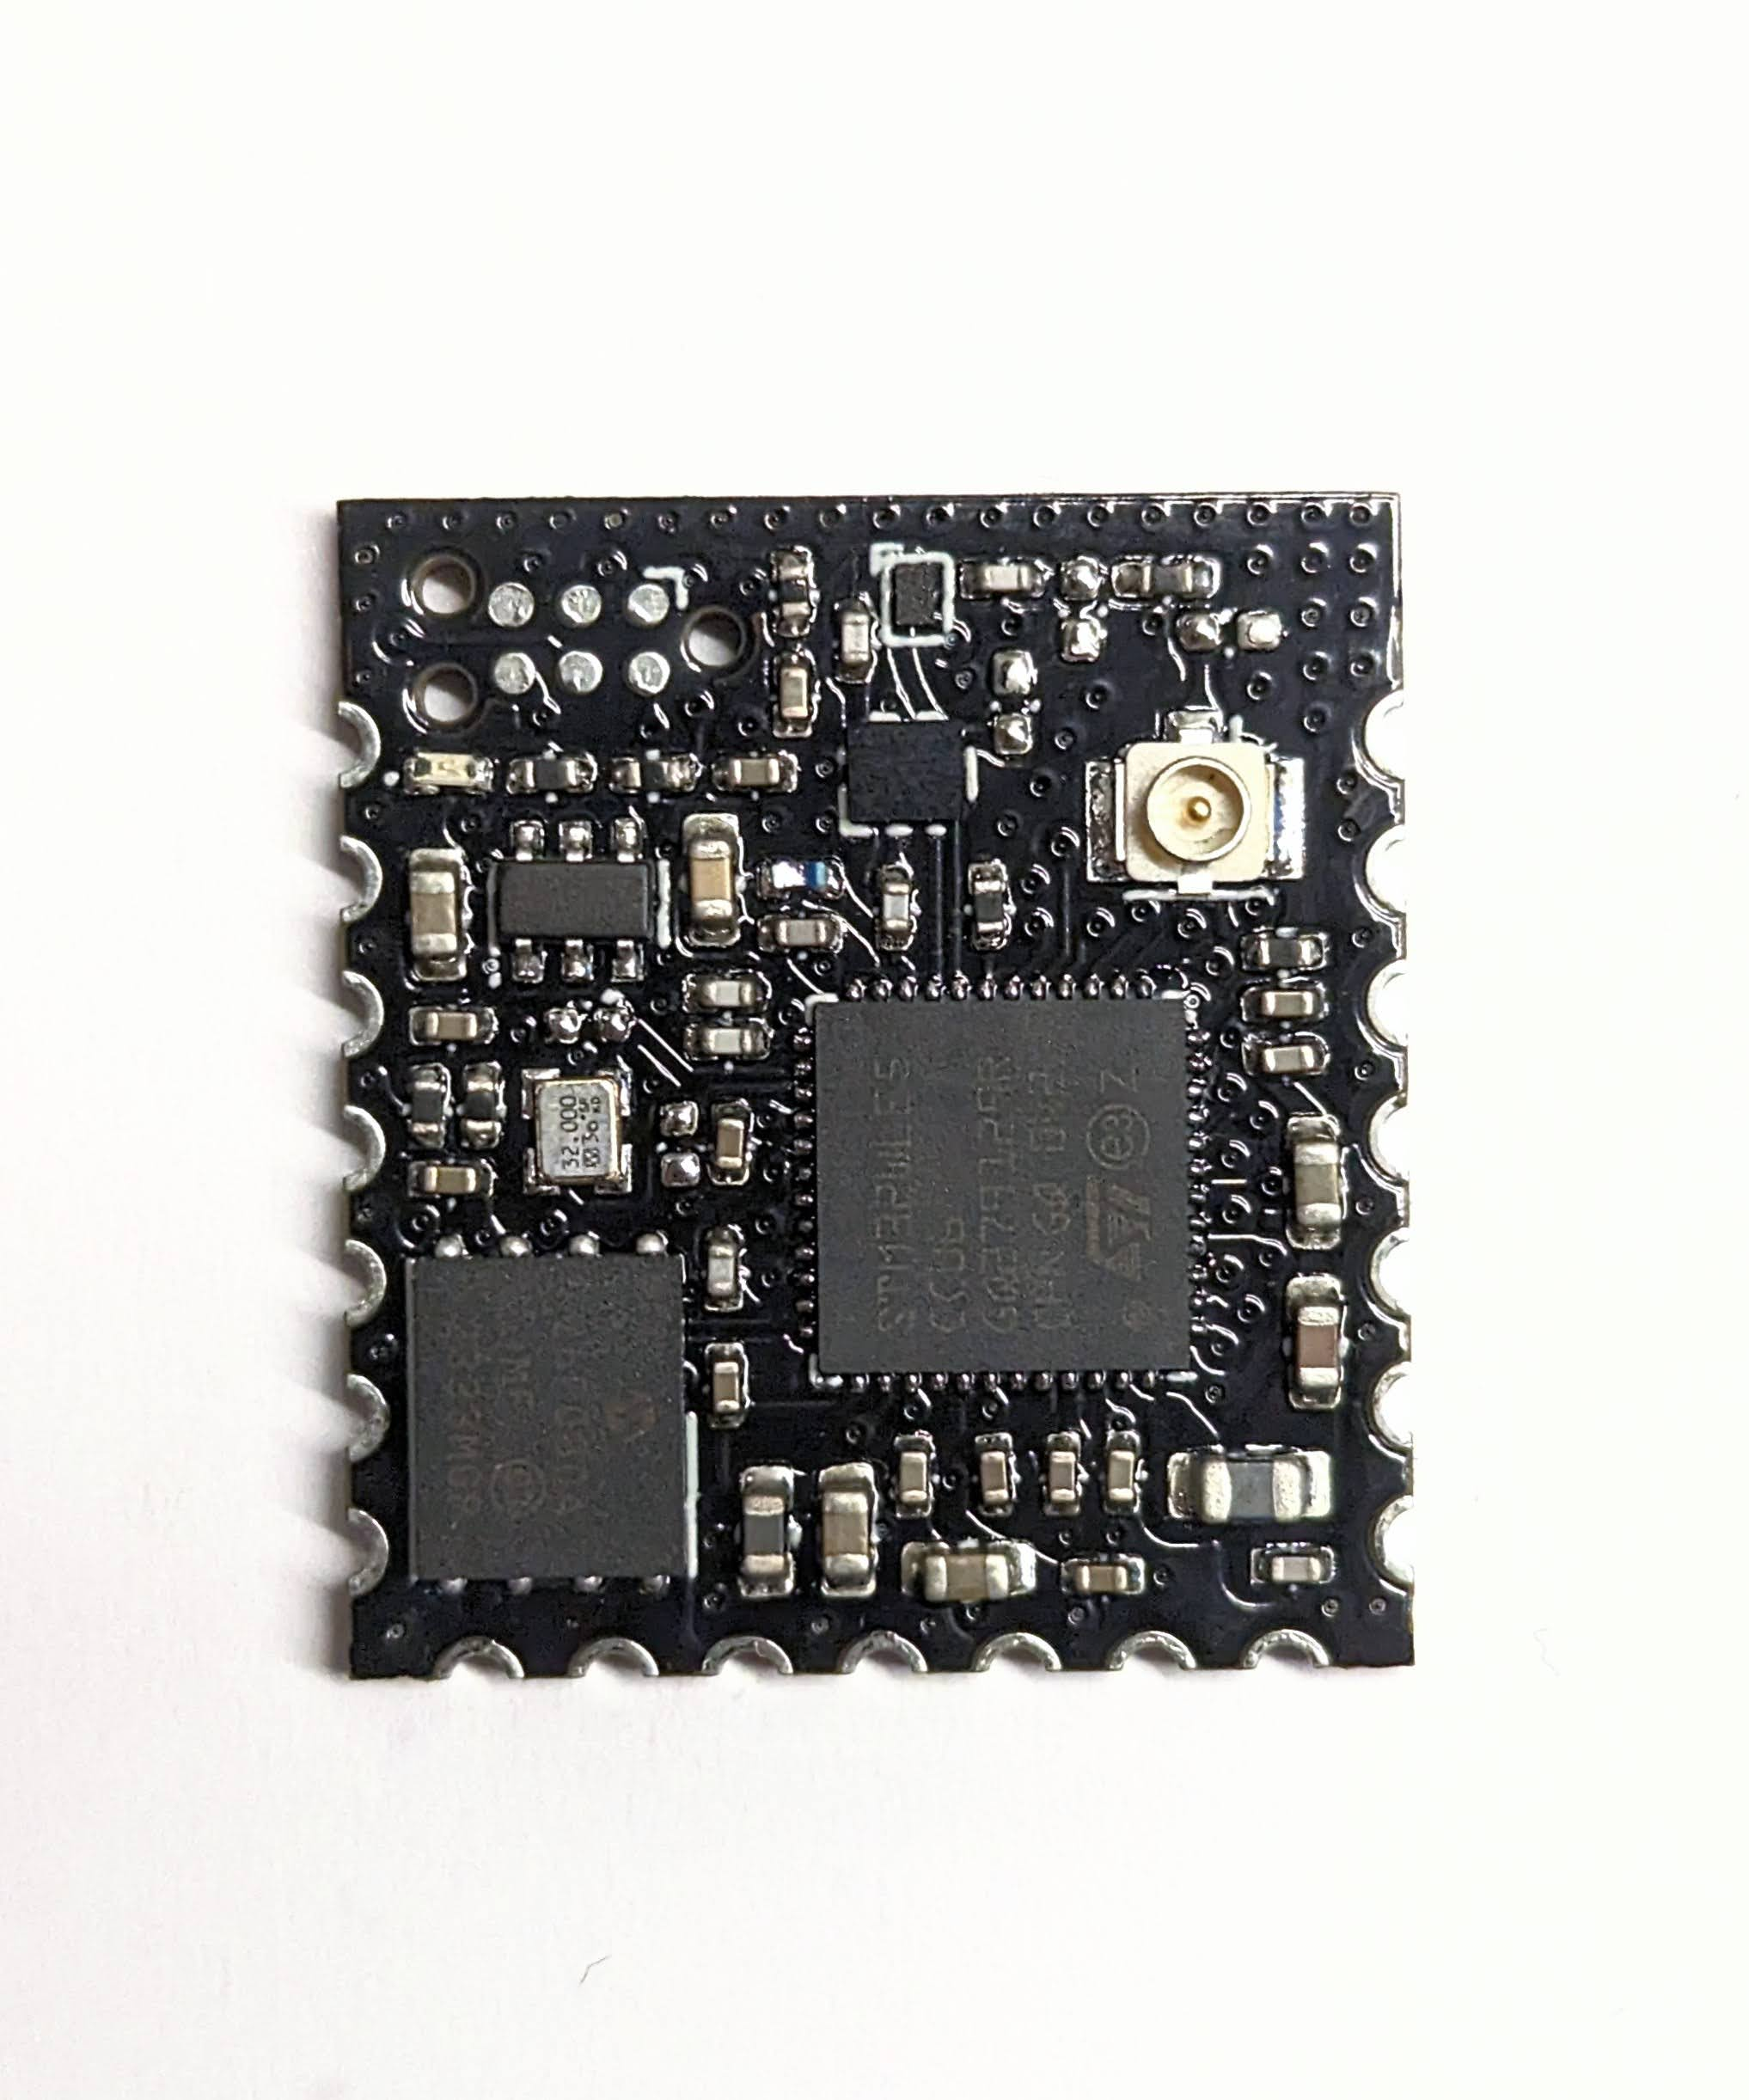
\includegraphics[width=\linewidth]{img/module.jpg}
    \end{figure}
\end{column}%
\end{columns}
\end{frame}


\begin{frame}{Výsledky: firmware}
\begin{columns}[T]
\begin{column}{.35\textwidth}
    \begin{itemize}
        \item Výběr prostředí a\,nástrojů
        \item Adaptace na vlastní HW
        \item Základní implementace procesu aktualizace
    \end{itemize}
    Zbývá
    \begin{itemize}
        \item Bootloader
        \item Adresace více modulů
        \item Zabezpečení
    \end{itemize}
\end{column}%
\hfill%
\begin{column}{.70\textwidth}
    \begin{figure}[h]
        \centering
        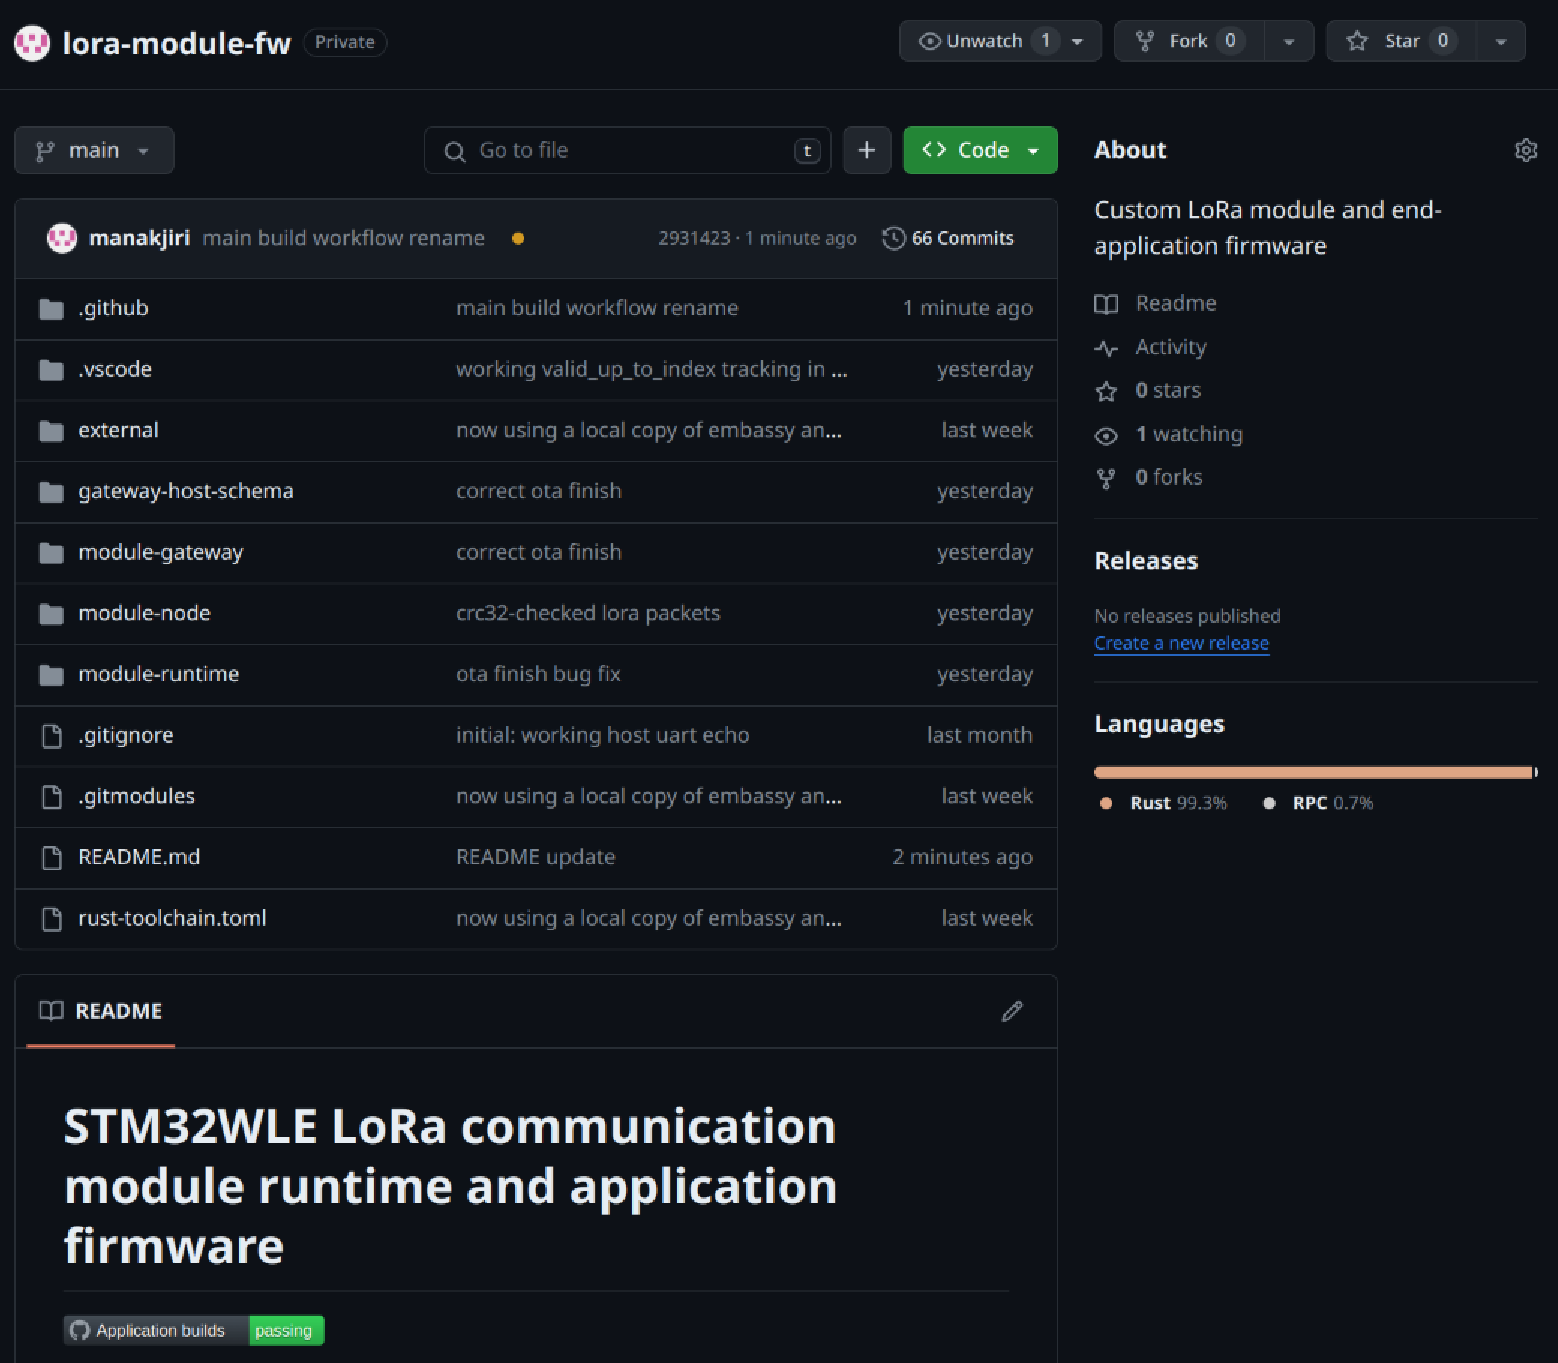
\includegraphics[width=\linewidth]{img/firmware.png}
    \end{figure}
\end{column}%
\end{columns}
\end{frame}


\begin{frame}{Výsledky: ukázka OTA přenosu}
\begin{figure}[h]
    \centering
    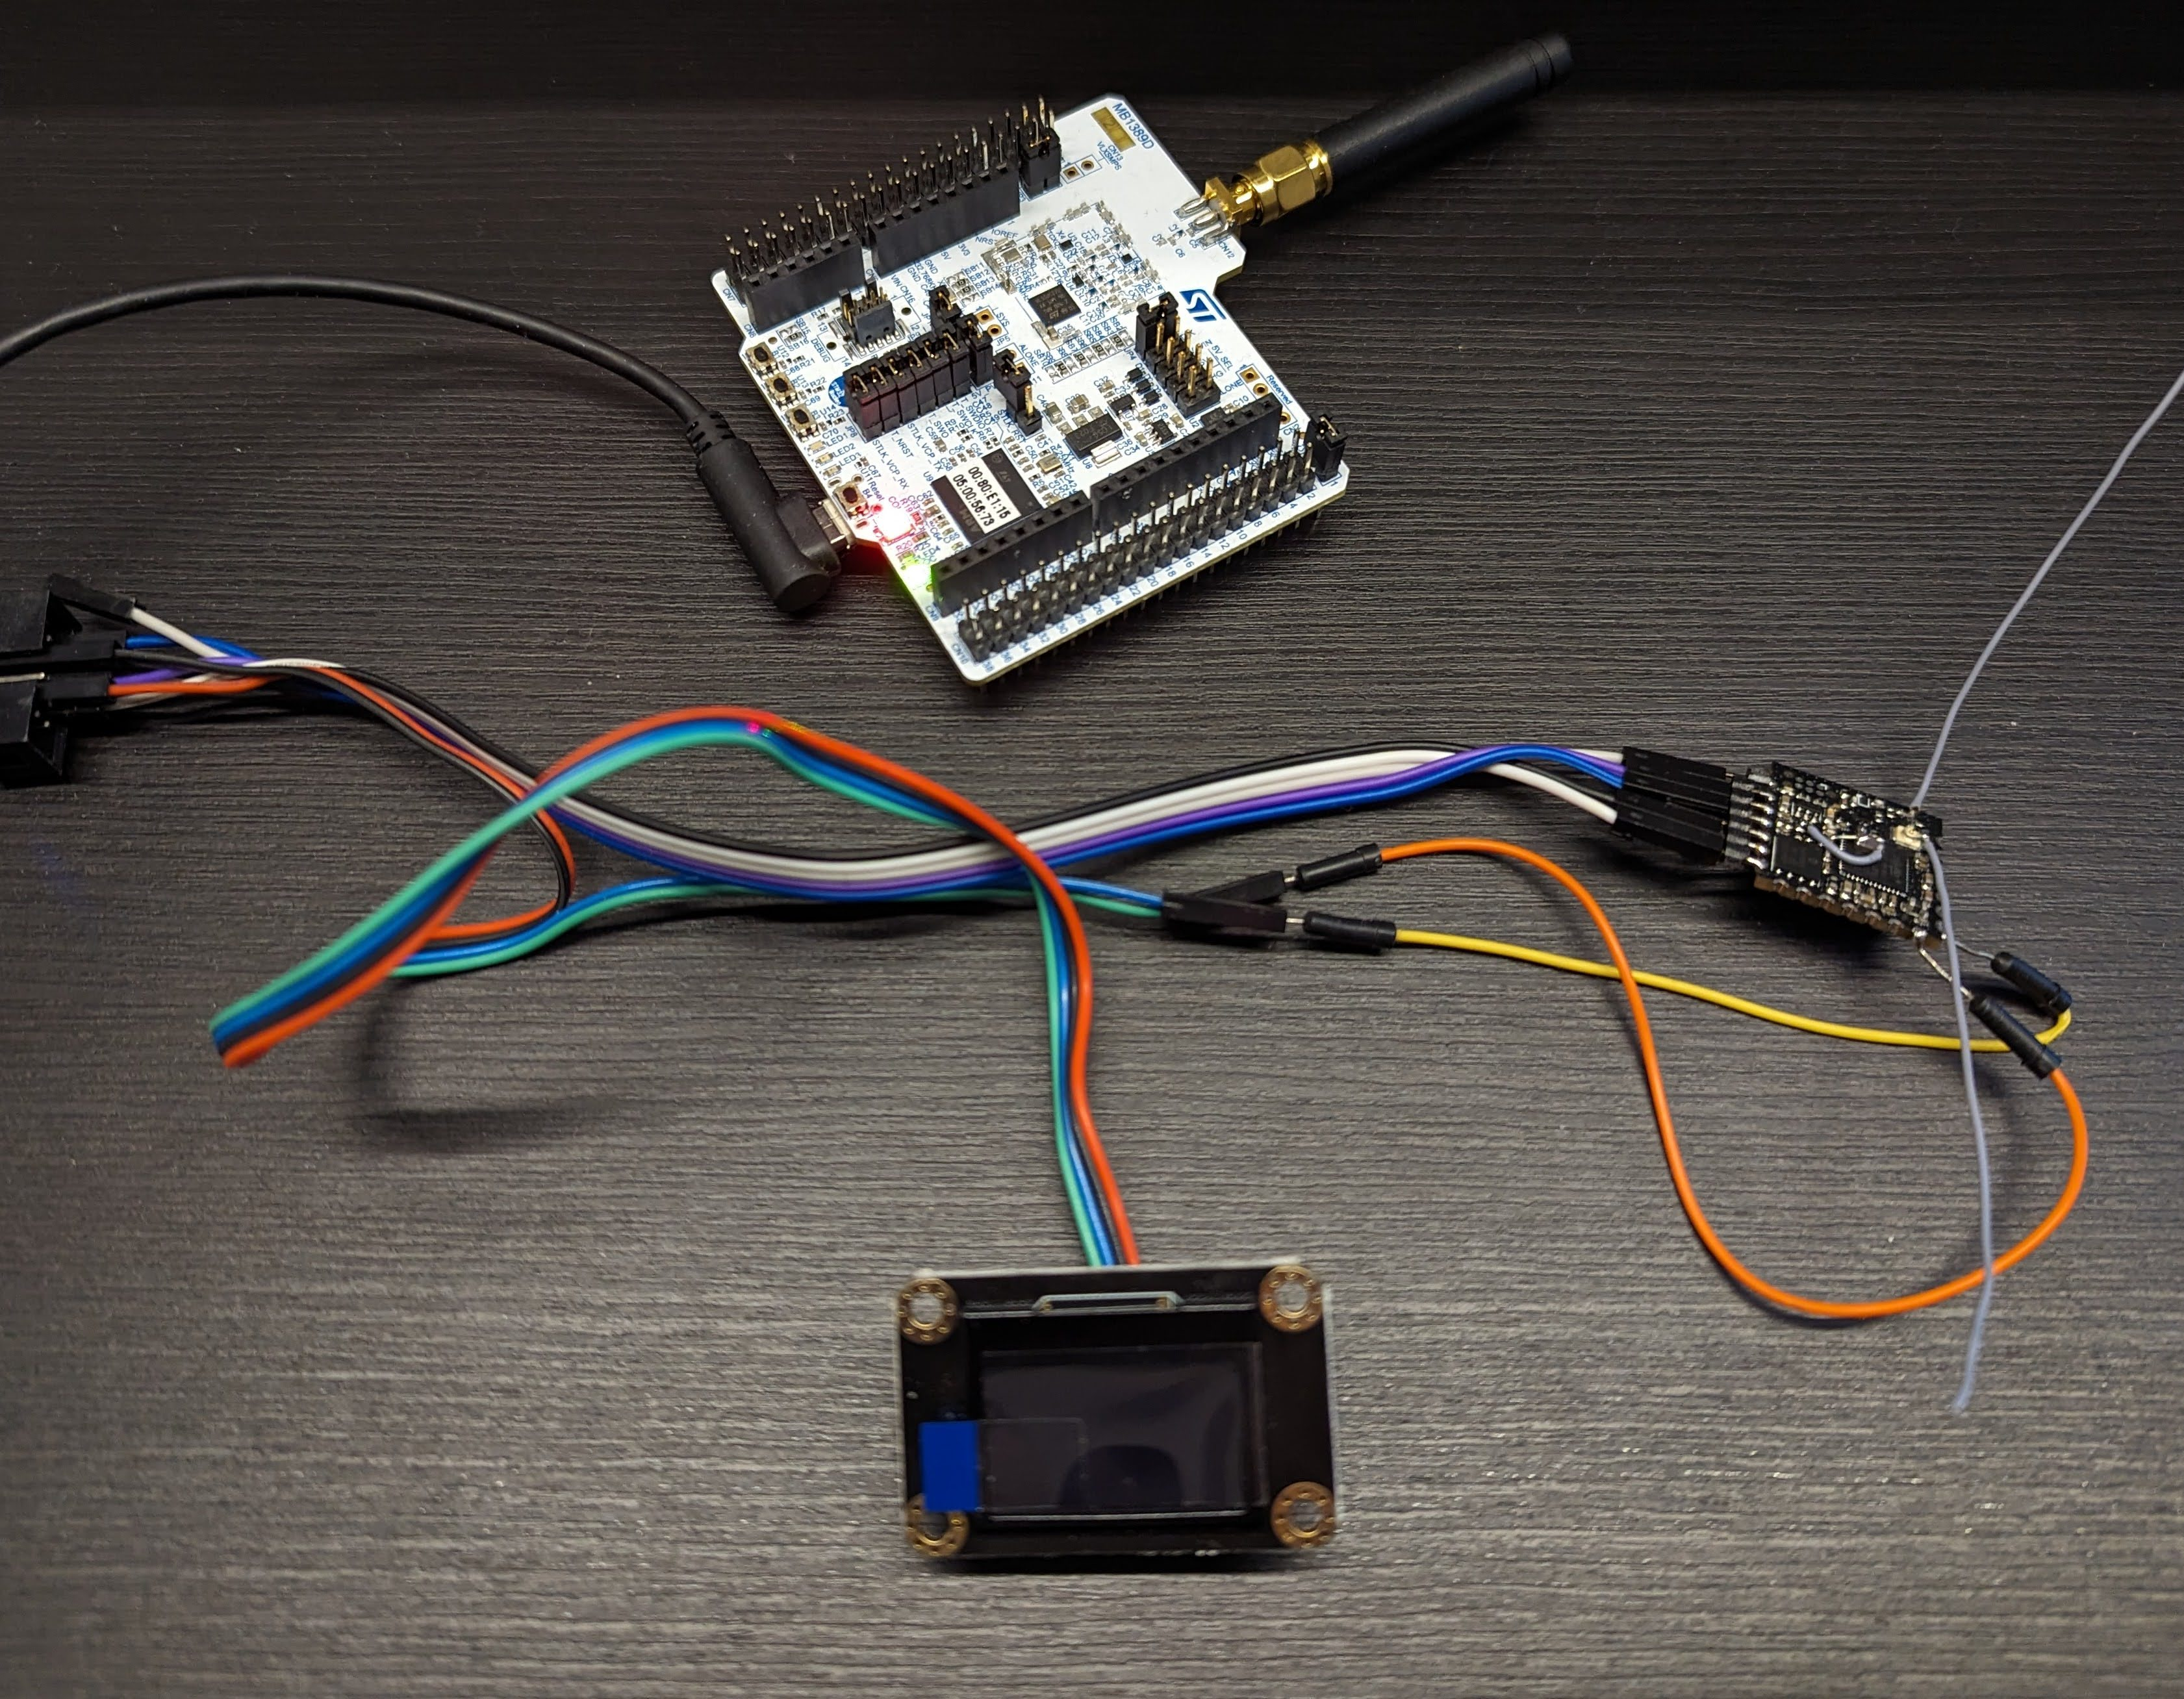
\includegraphics[width=0.8\linewidth]{img/demo-setup.jpg}
\end{figure}
\tinyline{\url{https://manakjiri.cz/assets/content/videos/lora_ota_demo.mp4}}
\end{frame}


\begin{frame}{Shrnutí}
\begin{itemize}
    \item Hardware - prototyp dokončen, další revize v přípravě
    \item OTA aktualizace - přenos funguje, chybí bootloader
    \item Napájení - navrženo dle požadavků, nutno uskutečnit samotná měření
\end{itemize}
\end{frame}

\end{document} 
